
\chapter{Steganography methods}


\section{Least Significant Bit(LSB) Insertion}
\begin{multicols*}{2}
\subsection{Sequential}
\setlength\columnsep{20pt}

Least Significant Bit or LSB is by far the most used method when talking about any type of steganography. Given that the smallest unit a computer can understand and process is usually a byte, altering only the least significant bit will not change the transmitted information in a noticeable way to any external parties. It is much easier to showcase what a byte contains and what the LSB change implies and how it works. A byte contains 8 bits, so this means that the values a byte can take range anywhere from 0 to 255 (inclusive)\footnote{This is the case for unsigned bytes, but given that we are talking about a method that only deals with the least significant bit, we can safely ignore the most significant bit, also known as the sign bit.}. Let's assume that we have an array of 4 random values in consecutive memory : 217, 127, 100, 62 (all values are in decimal), each stored on exactly one byte, and that we want to hide our grade in Numerical Analysis from our parents (in this case a 3) using a LSB substitution. The process would be something like this :

\begin{figure}[H]
    \centering
    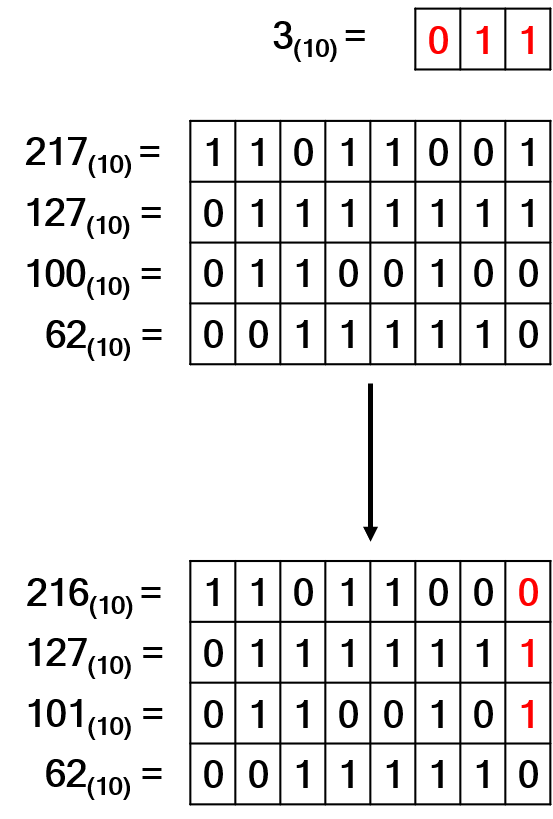
\includegraphics[width=2.8cm,keepaspectratio]{pics/how_lsb_works}
    \caption{How the sequential Least Significant Bit change works}
    \label{LSB}
\end{figure}

As we can see from Figure \ref{LSB}, we have succesfully altered the least significant bit of the first 3 bytes of the stream in order to hide our grade : 217 became 216 when we changed the last bit from 1 to 0, 127 was unchanged because it already had the last bit set, and the third byte became 101 after toggling the final bit. Furthermore, the rest of the stream (the fourth byte, 62) was not affected because we already hid the entirety of our secret message. While this is great because we only hide exactly as much as we need and not a byte more, we have a high risk of corrupting the hidden message in case our cover image gets compressed or loses even a single byte when sent over a network. Basically, we are trading data redundancy in order to get simplicity and efficiency.

Sequential LSB insertion is the simplest and most common way of embedding any kind of information into a byte stream that is then shared. It has been thoroughly discussed by a great deal of researchers and has been the subject of many papers where it was analyzed and benchmarked\cite{seeing-the-unseen}\cite{hide-and-seek} . Being the most popular technique also means that any flaws the method has are widely documented and showcased. Steganalysis\footnote{Steganalysis is the study of steganographic methods, including but not limited to : differences in file sizes or in color histograms, secret message redundancy, embedding capacity and performance etc.} performed on outputs created using this algorithm has shown that it is unreliable to stay undetected if an outside party intercepted the message containing the cover file\cite{attack-on-steganography}. Furthermore, doing a simple reverse engineering on the algorithm reveals even more issues with this naive encoding : if a single bit that is part of the secret message was flipped from the cover file byte stream, the message would become corrupted and the original secret would be lost forever. This means that sequential LSB insertion is not resistant at all to any form of lossy compression where some of the original data may be lost in order to reduce the used disk space because it would lose most, if not all, of the embedded file information. 

Furthermore, it is extremely easy to compute the carrier storage, i.e. how many bytes we are able to hide into the cover file or in other words, the maximum size of the secret message that we can succesfully embed without losing anything while still keeping a covert profile. Assuming $CDS$ or Cover Data Size (how many bytes are actually used to store the pixel information, no metadata information or chunk headers or anything like that), then the $MMS$ or Maximum Message Size would be equal to

\[ MMS = [CDS \ / \ 8] \ bytes \]

or the integer part of CDS divided by 8. This should come as no surprise since sequential LSB is altering $1/8$ (an eighth) of each byte when embedding a bit of the secret information so the maximum capacity makes sense to also be $1/8$.


\subsection{Scrambling}
As documented earlier, sequential LSB insertion algorithm has a decent number of flaws so it was needed to develop some new techniques that are not relying as much on the cover file not losing a few bytes or undergoing a compression algorithm. In other words, it needed to introduce a few redundancies to ensure that the secret message wouldn't be lost as easily and that the message was not written in a sequential and direct order. They achieved this by not just changing the least significant bit in a sequential order, but by writing in an apparently random order (in simpler terms, scrambled) that could be reproduced by having the right key or by using the same algorithm in order to retrieve the embedded information. In this subsection we will discuss a few of the most common scrambling techniques and introduce a new one as well.

The most popular methods used for scrambling secret messages into various covers usually choose to simply ignore the entire data stream and only focus on a specific subsection and choose that as the carrier environment. After a smaller subsection is chosen (it can still be the entire actual data part of the cover, it's not an actual rule), we will have to generate the order in which we will write the message information. As mentioned before, this is derived using a key known only to the sender and the receiver that can be shared between the 2 parties using another transmission environment, preferably one that is encrypted and safe. The main logic is to use that passkey as a seed in a valid pseudo random engine when generating the order so that there are no collisions and that only the right key will produce the right order. 

There is also an option for when there is no safe method of transmitting a key and that is to scramble the secret message within a certain order that is not sequential. But as long as the receiver and transmitter have no way of communicating the algorithm used in embedding the message (can also assume this because they have no way of sharing the key), this option is useless but is still interesting to look into because they are a variation of the other mentioned option. Having no key to generate the order makes this option easier to showcase(since we don't have to also simulate a pseudo-random engine and a seed). Let's assume we have a byte stream of random data\footnote{Now the actual data meaning can be safely ignored because we only work on the LSB and we have seen in the previous chapter it does not alter the data in a significant way such that an intruder might notice something is wrong.} and we want to again hide a grade from our parents, in this case a 6 (or 110 in binary). Instead of hiding the grade sequentially, the bits will be hidden into the last bit of every third byte and it will end up looking something like this :

\begin{figure}[H]
    \centering
    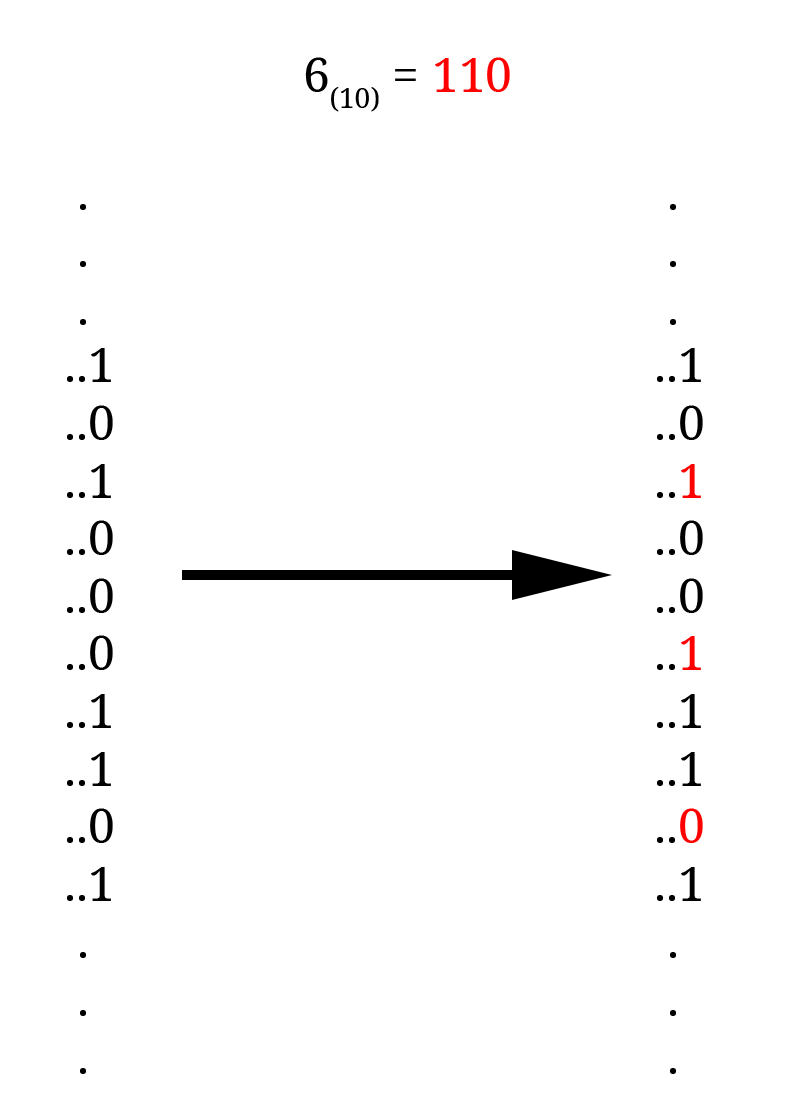
\includegraphics[width=5cm,keepaspectratio]{pics/scrambling_example}
    \caption{An example of scrambling LSB insertion}
    \label{Scrambled LSB}
\end{figure}

The key difference from sequential LSB insertion is that as long as the sender and receiver are aware of the used algorithm, any external parties will not be aware of the secret embedded message. Furthermore, this method has proven very useful because there are infinite ways of scrambling a message into the cover file without alerting any possible intruders and it ends up being an extremely hard guessing game for the attackers in their goal to extract the information.

The carrier capacity appears initially to be the same, but it is very important to remember that the scrambling algorithm used will usually work on a subset of the cover data bytes, not the entirety of it (just like in figure 2.2 we used only each third byte to store the information). Using the same notations as in the previous chapter we get that 

\[ MMS \leq [CDS \ / \ 8] \ bytes \]

so in most cases, the scrambled MMS will be smaller than the sequential MMS. However it is very important to note that this decrease in size comes with a great increase in data security and message safety.

This paper also introduces a new type of scrambling algorithm created by the authors that only works on lossless image formats that do not use any kind of interlacing when rendering the picture. It relies on scrambling the secret message into the image sub-blocks in a specific order that can only be deduced by having the right passkey. More information on this method is presented in chapter 3.2.1 after the introduction of image basics.


\section{Metadata encoding}
The word metadata was formed from combining the word "data" with the prefix "meta-" and is used to describe a special type of data that has information about other types of data\cite{metadata-origin}. In simpler terms, it means "data about data" and it keeps the same meaning in the digital world. It is much easier to visualize and understand the concept of metadata using a simple example : let's take a picture stored on a computer.

\begin{figure}[H]
    \centering
    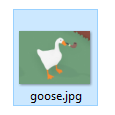
\includegraphics[width=2.3cm,keepaspectratio]{pics/goose_file}
    \caption{A simple image file}
    \label{Goose Image File}
\end{figure}

As noted in the introductory chapter, every file can be seen as a byte stream. However it is very important to keep in mind that those bytes don't represent only the image data, the pixels seen on the screen, they are much more. They also contain information about the camera used to take the photo, the location where it was taken, when the file was created, when it was modified, etc. All of the aforementioned information forms the metadata. It varies from file format to file format where they store this information in the byte stream, how many bytes are allocated for each piece of information or if it even has any effects on the actual file data. Most of the time metadata fields are only parsed by the renderer software and are mostly hidden to the user, but there are a few ways of viewing the information: 
\begin{itemize}
  \item using a hex editor to view the raw bytes of the file and then mapping those bytes to the publicly available file format specifier - an international approved paper which specifies the meaning of the bytes in the file binary stream
  \item using the operating system to view more properties about the file, not just the actual data interpreted and displayed to the end user
  \item using a third party tool which already knows the mapping and meaning of each sequence of bytes in the file binary stream and can succesfully parse the metadata
\end{itemize}

\begin{figure}[H]
    \centering
    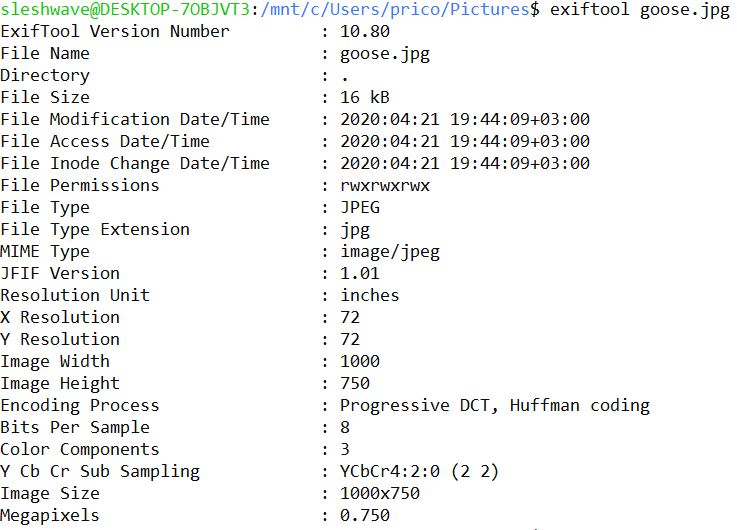
\includegraphics[width=8cm,keepaspectratio]{pics/exiftool_file_metadata}
    \caption{Example of using a tool to read file metadata}
    \label{Goose Image File Metadata using Exiftool}
\end{figure}

The focus of this sub-chapter will be on the metadata fields that don't necessarily have any important effect on the data representation and theoretically could be altered, such as any comments from the author or any contact information. In the case of an image, changing important metadata fields such as the width or height of the picture are not very covert methods of embedding any information at all, proving that not all fields are equally important. We are left with the more \textit{useless} metadata fields, but the good news is that most file formats allow these fields to have a variable size which is perfect for any steganographic purposes because it removes the size constraint of the secret message. While in theory this allows for $\infty$ MMS, there are a few limitations in place that significantly reduce that number: 
\begin{itemize}
  \item computers have a limited amount of storage space, in most modern day computers that would be about one terabyte. This means that the MMS will certainly be smaller than that.
  \item most file formats that allow metadata fields to be embedded in the byte stream of the file by an external party also have a sequence of bytes that indicates how long that metadata field is (how many bytes it contains). In most cases that sequence is 4 bytes long so this usually results in a MMS of $2^{4*8} = 2^{32} \approx 4.29\ gigabytes$.
  \item in the pursuit of keeping the existence of a secret inside the cover file as covert as possible, the MMS is again limited by the CDS. This happens because the size of the cover file is almost always displayed to any parties without any interactions and it needs to not raise any suspicions or attract unwanted attention to the actual contents of the file. To give an example, it would be very weird to see a simple image in FULL HD resolution have a size of two gigabytes and will almost certainly alert any intruders. It is extremely hard to say an exact MMS based on this limitation because it depends on the original cover file size and it should be relative to that number. It is recommended that $MMS \leq  50\% * CDS$.
\end{itemize}

In the end it is important to note that metadata secret encoding is the most trivial method of embedding secret information into different kinds of cover files. However, this method comes with a great cost: almost every single tool that specializes in extracting metadata will be able to detect and identify our message without too much hassle because the final cover file still has to respect the format specification.

\begin{figure}[H]
    \centering
    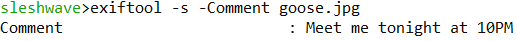
\includegraphics[width=8cm,keepaspectratio]{pics/metadata_message_identified}
    \caption{Example of message hidden in a file in the metadata section}
    \label{MetadataMessageExample}
\end{figure}

\section{Unused space embedding} \label{Unused_Space_Chapter}
Usually most file formats and even internationally approved and used protocols such as the TCP/IP have unused bits or bytes in their composition, either for future proofing the format in the form of reserved space or simply to serve as padding space mainly present to help the associated parsers. 

One well known example of this is found in the BMP file format which appears only in the cases where the width of the image is not a multiple of 4. The standards specify that in this situation there needs to be added the right amount of bytes to fill so that the width will be divisible by 4. So if an image has a resolution of 1920x1080 (the width is the first number), there won't be a need for any padding bytes because 

\[1920 \% 4 = 0\]

On the other hand, if the image had a resolution of 125x100, we would instead have

\[125 \% 4 \neq 0 \implies 4 - (125 \% 4) = 4 - 1 = 3\ bytes\]

to serve as a padding for each pixel line, ending up in a total of $100 * 3 = 300$ bytes of simple, raw, unused space that most BMP parsers will ignore because they know that data is meaningless. 

Another very good example is in the case of the IPv4 packet header which has a reserved bit in the flags subsection, or to be more precise, the 49th bit. According to RFC3514\cite{RFC3514} it is meant to be a security bit representing the true intent of the packet (GOOD or EVIL), however it is important to note that it was an April Fools informational memo and it is most likely that altering this bit will still go undetected by any kind of firewall or intrusion prevention system.

\begin{figure}[H]
    \centering
    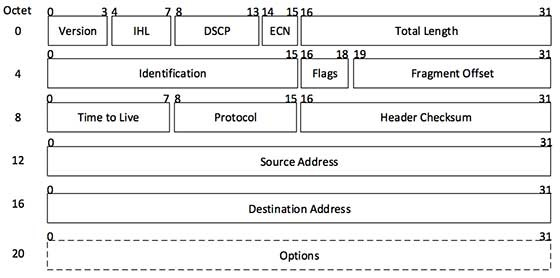
\includegraphics[width=8cm,keepaspectratio]{pics/ip_packet_specifier}
    \caption{The structure of an IP packet}
    \label{IP_Packet_Specifier}
\end{figure}

Given the IP packet header specifier represented in Figure \ref{IP_Packet_Specifier} it becomes trivial to alter the first bit of the flags section to the current bit of a secret and then over multiple sent packets to actually send the message in one of the most covert ways possible. Furthermore, it is very important to note the contribution done by Kamran Ahsan and Deepa Kundur in their 2002 article entitled "Practical Data Hiding in TCP/IP"\cite{practical_data_hiding_tcp_ip} because they also achieve the ability to send covert information by taking it one step further: using IP packet headers that may actually even be in use and by using Chaos Theory in the values of the Identification field sent over.

However, there is still one very important spot left in a file's byte stream where the secret message could easily be hidden: at the end of it. Most file formats either have specially crafted headers that announce the end of the file\footnote{One good example is the PNG format which has an IEND header and a couple of other information to mark that the image data has ended and that there is nothing left that is relevant to the parser. More information regarding this format is available in chapter \ref{BMP_Explained_Chapter}.} or have a few bytes reserved at the beginning of the file that mark the length of the data\footnote{This method is found in BMP or WAV file formats usually, it is very simple and easy to work with for parsers. More details in later chapters.}. It is important to note that both of these methods basically produce the same result technically speaking: a superior margin, a maximum amount of bytes that are to be read and interpreted by the parsers that contain the data relevant to the current file. After that region has ended, it is a free-for-all memory territory for secrets to be embedded. The same limitations from the previous chapter still stand, it is recommended that $MMS \leq  50\% * CDS$ in order to remain as covert as possible while still exfiltrating data.

\begin{figure}[H]
    \centering
    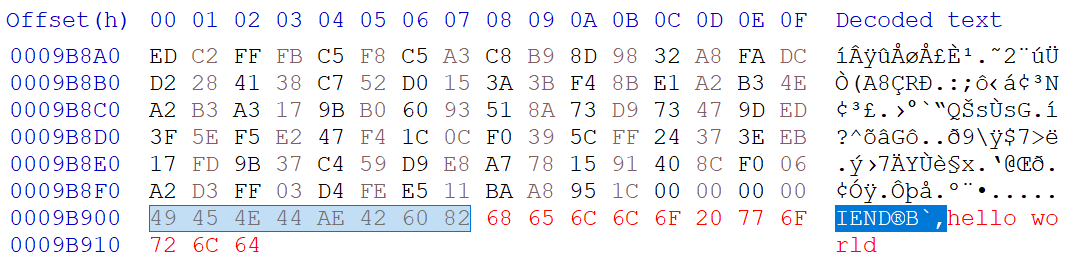
\includegraphics[width=9cm,keepaspectratio]{pics/secret_after_file_ended}
    \caption{Simple example of hiding a note after a file has ended}
    \label{secret_after_file_ended}
\end{figure}



\end{multicols*}